\section{Overview}

Plan merging involves the integration of multiple paths derived from various agents to construct a plan. Individual Path Finding~\ref{sec:ipf} which represent the computation part of multiple paths dor agents, can be a constituent of Plan Merging but it is not necessary.

The second step of Plan Merging is Path Selection~\ref{sec:pathselection}. Path Selection having the goal of identifying paths that closely resemble valid solutions to the problem at hand. However, it necessitates the construction of conflict-free set of path, which is computationally intensive, especially with a lot of agents and a lot of paths. This is where we incorporate Path Elimination to reduce the number of paths by eliminating potentially ``problematic'' paths using conflict-based strategy.

The final stage of Plan Merging involves obtaining a solution, which can be achieved by utilizing the pre-computed paths provided by Path Selection, by using the paths in their original form, or by employing the delineation of the pre-computed paths as a subgraph in order to reduce complexity for a MAPF algorithm.


The following figure~\ref{fig:overview} shows the different part of Plan Merging, having in order, Individual Pathfinding, Path Selection and Solving.

\begin{figure}[H]
    \centering
    \caption{Overview of the thesis}\label{fig:overview}
    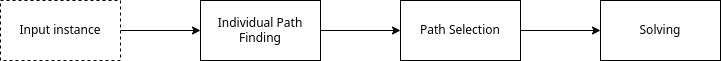
\includegraphics[width=\widthimg]{img/overview.drawio.png}
\end{figure}

